%!TeX root = 4-ml.tex
\documentclass[main]{subfiles}

\begin{document}

\chapter{Statistical Learning of Adsorption Properties}
\vspace*{-1\baselineskip}

\section{Machine Learning Models}

Machine learning (ML) models have been widely used to characterize adsorption, transport, catalytic or mechanical properties, just to cite a few. It can in some cases replace very time consuming simulations with simpler calculation of key descriptors that can help the model predict the desired properties. In other cases, it is used to describe the structure--property relationships learned by the ML model. However,machine learning is not a silver bullet, we cannot blindly apply it on any applications; it requires a thorough work on understanding the key variables that will improve the prediction. By using our work on the thermodynamic descriptors and our knowledge on the effect of pressure on the selectivity, we will build a machine learning model to characterize the separation of xenon from krypton at ambient pressure.

\subsection{From algorithm to machine learning}

To understand how machine learning, first, we need to understand how a computer accomplishes a task. The human operator plays a key role in the process --- after designing the solution through theoretical considerations, he needs to write down a list of instructions, called an algorithm, that specifies all needed actions given the circumstances so that the computer achieves the desired outcome. In physical or chemical sciences, these algorithms usually articulate the different components of a theoretical model, which can be an equation without analytical solutions, an analytical expression or a probabilistic problem, just to cite a few. The previous chapters typically presented such algorithms for the simulation of adsorption processes; for instance, the GCMC simulations are based on the statistical physics of the phase equilibrium between a gas phase and adsorption phase inside a nanoporous material, and a Monte Carlo model is used to reproduce the statistics associated to the grand canonical ensemble. The energy sampling algorithms, along with the Widom insertion, are also good examples of how the computer can help the theoretician model the systems under specific chemical and physical conditions. 

A machine learning model is also based on an algorithm, but the goal is very different from the above-mentioned examples --- it doesn't aim at giving all the details of the computation according to proven theoretical principles. As implied by the name, the ambition would be to learn underlying relations within the input data so that it performs the task itself. The machine learning (ML) algorithm is then the list of instructions that specifies how the machine is going to learn from the data. For example, clustering algorithms can distinguish different classes of elements within a disordered dataset so that new concepts emerge; this type of machine learning algorithm is called unsupervised learning because we do not predefine or pre-label the data and the machine helps us understand the underlying structure in the data. The class of algorithm we want to study is rather the supervised learning model, which learns from labeled data the relation between the label and the characteristics (called features or descriptors) from a given set of data points, and can predict the label from unlabeled data using the characteristics. For example, if we want to predict the weather of tomorrow, the model could use the past weather of similar dates to infer if it will rain tomorrow; the history of the weather  forms the features of the ML model and the future weather is the target variable or the label of the data.

To articulate the differences between a standard algorithm and an ML algorithm, let me introduce a fascinating board game called Go. This game is traditionally played with 2 players on a 19 by 19 board, where each player places black/white pieces to control the maximum of boxes. Based on these simple rules, different algorithms have been developed to make the computer play the game. The first Go program was written in the late 60s to mimic the pattern recognition of Go players when estimating the ``score'' through an influence function,\autocite{zobrist1970feature} and from the 80s to the beginning of the 21\ex{st} century the first Go programs capable of playing were releases. These programs were based on simple alpha-beta search algorithms that seeks at testing every possible move (while pruning the less promising ones); while they were working very well in other games like chess (IBM's Deep(er) Blue beat the world champion of chess in 1995), in Go these types of programs were only at the level of a novice player. The difference of performance lies in the combinatorics behind both games, the game of chess has a number of legal positions lower than $10^{47}$,\autocite{website_labelle} while for the game of Go there are approximately $10^{171}$ legal positions.\autocite{Tromp_2007,github_tromp_go} The state space to explore is incomparably greater and a boost in the computing power that improved the performance for computer chess is not going to make a difference for Go. A drastic reduction of the space to be explored is needed for a computer program to work. The biggest improvement came, when in 2007, Coulom introduced a Monte Carlo tree search.\autocite{Coulom_2007} This algorithm uses heuristics to distinguish between bad a good move according to human perception of the game, a probability of selection is assigned to the moves according to their potential (policy), potential moves are randomly picked according to this probability; the average outcomes associated with a parent move gives the value of the move. The computer Go is now more efficient in the evaluation of the moves using a Monte Carlo sampling, and it can now play with average amateur players, but it is nowhere near surpassing them. Up until now, the algorithms are based on human knowledge that the programmer implements directly in the computer using machine instructions. Statistics and randomness are used to orient the machine towards the best moves and reduce their predictability, but the statistics that identifies the moves are based on human heuristics that are usually not generalizable. The big revolution brought about by machine learning in the field aims at better evaluating these statistics using the data from already played games. By using a dataset of 30 million moves, the Alpha Go is based on the same Monte Carlo tree search framework but it replaces the formulas behind the probability of searching a move by a machine learning model called the ``policy network'' and the one behind evaluating the confidence in winning of the position by a value ``network''.\autocite{Silver_2016} Alpha Go was the first computer program to beat a world champion in 2016. One year later, to further emancipate from human knowledge, an improved version, Alpha Go zero generates its own data by playing games against itself to train a similar machine learning structure than presented before. This new version beats 100 times out of 100 the former version,\autocite{Silver_2017} which marks a new era of domination of computer go over the best player in the world, and the defeat of another top player just confirms the advent of this new era. 

In this example, we can see how the machine learned the value of each moves by compiling the knowledge of huge datasets in a deep neural network. The main difference between conventional approaches to algorithmic and machine learning is very well illustrated in the previous example; the goal is not to tell the computer how to play using player knowledge implemented in formulas and explicit instructions, but it is to give an explicit framework with flexible parameters that the model needs to learn using a database. In other words, the parameters of a model are fitted to match the values of a database, while being capable of generalizing in situations outside of the database (this notion of generalizability will be further discussed in the following sections). In this section, the goal is not to give a complete overview of all existing models but rather to introduce the main concepts of ML through the example of the model we will use for our problem of selectivity performance prediction.

\subsection{Introduction to supervised learning}

In this thesis, we will focus on the most common way of statistically learning from data, which is the supervised learning. As previously introduced, supervised learning corresponds to the extraction of a relationship between the labels of a set of data points and some of their known characteristics or features. This relationship can be called the model or the predictor and should ideally generalize to similar but unseen data. In this section, we will formalize the goal of the learning algorithm when given a set of labeled data in order to introduce more complex notions in machine learning like the bias--variance trade-off and also more specific models that will be used in this chapter like the tree-based models.

\subsubsection{Mathematical considerations}

\todo{HERE}
Le ML appliqué à l'apprentissage supervisé, c'est donc avant tout l'art d'exploiter des données: on note $\mathcal{D}_{n}:=((X_{1},Y_{1}),...,(X_{n},Y_{n}))$ un {jeu de données} comportant $n$ observations indépendantes et identiquement distribuées d'une loi $\mathcal{P}$, où $X_{i}$ est un vecteur de $\mathbb{R}^{p}$ ($p$ étant un entier naturel non nul) et $Y_{i}$ appartient à un ensemble $\mathcal{Y}$ de données (numériques ou non). On note $\textbf{X}:=(X_1,\ldots,X_n)$ et $\textbf{Y}:=(Y_1,\ldots,Y_n)$. Un \emph{prédicteur} est alors une fonction $f$ définie de $\left(\mathbb{R}^{p}\right)^n$ dans $\mathcal{Y}^n$. On définit ensuite une \emph{fonction de perte} $\mathcal L$ de $\left(\mathcal{Y}^n\right)^2$ dans $\mathbb{R}_{+}$: $\mathcal L(\textbf{Y}',\textbf{Y})$ représente alors le coût d'avoir prédit $\textbf{Y}'$ au lieu de $\textbf{Y}$. En particulier, le \emph{risque d'un prédicteur}, à savoir ${R(f(\textbf{X}),\textbf{Y}) = \E{\mathcal L(f(\textbf{X}),\textbf{Y})|((X_{1},Y_{1}),...,(X_{n},Y_{n}))\sim\mathcal P}}$ représente le coût d'avoir prédit $f(\textbf{X})$ au lieu de la valeur observée $\textbf{Y}$. Notons $(Y_1',\ldots,Y_n'):=f(\textbf{X})$ les valeurs de $(Y_1,\ldots,Y_n)$ prédites par le programme de ML à partir des données $\textbf{X}$. L'objectif de l'apprentissage supervisé est alors de choisir le prédicteur $f^*$ rendant ce risque minimal: autrement dit, on doit avoir ${f^*=\underset{f\in\mathcal F\left({(\mathbb{R}^p)}^n;\mathcal Y^n\right)}{\text{arg min}} R(f(\textbf{X}),\textbf{Y})}$. \vspace{-13pt}En particulier, lorsque $(Y_1,\ldots,Y_n)$ est un jeu de données binaires (lorsqu'on a $\mathcal Y=\{0,1\}$), la fonction de perte est définie par $\ell(\textbf{Y}',\textbf{Y})=\dfrac{\mathds 1_{Y_1\ne Y'_1}+\cdots+\mathds 1_{Y_n\ne Y'_n}}{n}$ en général: on calcule la fréquence des mauvaises prédictions au sein du jeu de $n$ données. On peut alors prouver que l'estimateur optimal $f^*$ vérifie $f^*(\textbf{X})=\mathds 1_{\E{\textbf{Y}|\textbf{X}}\geq 1/2}$. Mais comme on ne connaît généralement pas avec précision la loi de $\mathcal D_n$, il conviendra de proposer un estimateur $\widehat{\gamma}(\textbf{X})$ de $\E{\textbf{Y}|\textbf{X}}$. 

\todo{compare to the optimization of molecular structure in an \emph{ab intio} simulation. Find a minimum, gradient descent}

The Elements of Statistial Learning\autocite{Hastie_2009}

\todo{introduce what it means for linear regression}

\todo{L1 and L2 regularization lasso ridge / elastic net}
Tikhonov

\todo{cross validation, overfitting, hyperparameter optimization}





\subsection{Tree-based models}

\subsubsection{Regression tree}

\subsubsection{Random Forest}

Bagging

\subsubsection{Gradient Boosting}


random forest 
boosting
eXtreme Gradient Boosting

\subsubsection{Hyperparameters}

\todo{compile all hyperparameters}

We used the training data to perform a random search of hyperparameters, with 5-fold cross-validation to evaluate the root mean squared errors (RMSE) of the model. The range of search explored for each hyperparameter is made available in the SI. After this search, a set of optimal hyperparameters were identified that give an average RMSE of \SI{0.36}{\kilo\joule\per\mole}; we used it to build our final model. A convergence plot of the model performed using 5-fold cross-validations is given in Figure~S6. Given this configuration, the model is tested on the prior defined test-set and interpretation tools are used to better understand the structure-property relationships in play.

\section{Prediction of the Ambient-pressure Selectivity}

Simon et al. published one of the first articles on an ML-assisted screening approach for the separation of a Xe/Kr mixture extracted from the atmosphere.\autocite{Simon_2015} Their model's performance was highly relying on the Voronoi energy, which is basically an average of the interaction energies of a xenon atom at each Voronoi node.\autocite{Rycroft_2009} To rationalize this increase in performance, we regarded this Voronoi energy as a faster proxy for the adsorption enthalpy. By comparing it to the standard Widom insertion, we found that although it is faster, it is less accurate; and we developed a more effective alternative, the surface sampling (RAESS) using symmetry and non-accessible volumes blocking.\autocite{Ren_2023} Recently, Shi et al. used an energy grid to generate energy histograms as a descriptor for their ML model, which gives an exhaustive description of the infinitely diluted adsorption energies,\autocite{Shi_2023} but can be computationally expensive.

All the approaches described above can have good accuracy in the prediction of low-pressure adsorption (i.e., in the limit of zero loading) but are not suitable for prediction of adsorption in the high-pressure regime, when the material is near saturation uptake. While this later task is routinely performed by Grand Canonical Monte Carlo (GCMC) simulations, there is a lack of methods at lower computational cost for high-throughput screening. To better frame our challenge, in this work we are essentially trying to predict the selectivity in the nanopores of a material at high pressure, where adsorbates are interacting with each other, while only having information on the interaction at infinite dilution. The comparison between the low and high-pressure cases gives key information on the origin of the differences of selectivity. For instance, we have previously shown that selectivity could drop between the low and ambient pressure cases in the Xe/Kr separation application, and it was mainly attributed to the presence of different pore sizes and potential reorganizations due to adsorbate--adsorbate interactions.\autocite{Ren_2021}

In this section, we combined a grid-based approach with core components of our previously developed RAESS algorithm~\autocite{Ren_2023} to design a new adsorption energy sampling technique. Moreover, a statistical characterization of the pore size and energy distributions has been performed to inform the model on a potential selectivity drop. By combining these two approaches, we propose a set of useful ML descriptors for fast and accurate ambient-pressure selectivity prediction, and we highlight its performance on the case of xenon/krypton separation in the CoRE MOF 2019 database\autocite{Chung_2019}.\todo{ref previous chapter}


\subsection{Components of the ML model}

\subsubsection{The machine learning model}

We chose to use eXtreme Gradient Boosting (XGBoost) as the machine learning framework for our predictive model because of its accuracy, efficiency and simplicity of use. Its performance has long been proven since 17 out 29 Kaggle challenge winning solutions were based on this algorithm in 2015. The XGBoost system is highly scalable and parallelized, which gives very fast model training.\autocite{chen2016xgboost} Compared to more standard tree-based algorithms such as random forest (commonly used in the field~\autocite{Simon_2015}), the boosting component of the algorithm means that it learns from previous mistakes and puts higher weights on the problematic data points, hence improving the accuracy of the final ML model.

In the next sections, we introduce new descriptors for nanoporous materials, as well as new concepts of feature engineering based on energy and pore size histograms. The ML features presented have been selected by progressively filtering out the less influential ones on the accuracy of the final model, see the complete list in Table~S1-3 of Supporting Information (SI). The influence or importance is defined later in a section dedicated to the interpretation of the model. The hyperparameters of the model were fine-tuned using random searches to design the best performing final model. Finally, the influence of the preselected descriptors on the final model is interpreted using a unified approach.

\subsubsection{Target variable}

We want to predict the Xe/Kr ambient-pressure selectivity faster than standard techniques. To obtain reference values (ground truth), we used the Raspa2 software\autocite{dubbeldam2016} to run grand canonical Monte Carlo (GCMC) calculations of 20-80 Xe/Kr mixtures at \SI{298}{\kelvin} and \SI{1}{\atm} on our cleaned database. The van der Waals interactions are described by a Lennard-Jones (LJ) potential with a cutoff distance of \SI{12}{\angstrom}. The LJ parameters of the framework atoms are given by the universal force field (UFF),\autocite{rappe1992} and the guest atoms (xenon and krypton) have their LJ parameters taken from a previous screening study.\autocite{Ryan_2010} The study only focuses on a given Xe/Kr composition usually obtained by cryogenic distillation of ambient air~\autocite{kerry2007industrial} as a first step towards predicting other mixtures at different physical conditions (\emph{e.g.} Xe/Kr mixtures out of nuclear off-gases). In the broader scope, this methodology could be adapted to the desired application with some tweaks on the descriptors calculation (\emph{e.g.} \ce{CO2}/\ce{CH4} separation).

We decided to use a logarithmic transform of the selectivity instead of the raw value because we are more interested in the order of magnitude of the selectivity values than to predict the higher values of selectivity --- an ML model that predicts selectivity values can lower down the errors by focusing the prediction more on the higher values than the lower ones. By focusing on the logarithmic transform of the selectivity, we can better separate the different orders of magnitude of the selectivity values. This approach distributes more evenly the efforts on all the different values of selectivity. Moreover, this logarithmic transform is related to a thermodynamic quantity that we elaborate later in the section~\ref{sct:thermo}; it can therefore be easily compared with the energy descriptors we introduced in this article.

\subsubsection{Database and data preparation}

To test our methodology on a set of realistic MOFs, we chose to screen the 12,020 all-solvent removed (ASR) structures of the CoRE MOF 2019 database\autocite{Chung_2019}. After removing the disordered and the non-MOF structures as well as the ones with a large unit cell volume of \SI{20}{\cubic\nano\meter}, we obtained a set of 9,748 structures. Then we analyze the string information given by the Zeo++ software\autocite{zeopp_Willems2012} to reduce the number to 9,177 by removing the structures that are not tridimensional, where solvents are still detected (wrongly classified in ``all solvent removed’’), or where the metal is radioactive or fissile (e.g., Pu-MOF TAGCIP\autocite{Diwu_2010}, Np-MOF KASHUK\autocite{Martin_2017}, U-MOF ABETAE\autocite{Jouffret_2011} or Th-MOF ASAMUE\autocite{Liang_2016}) --- this can be a source of risks in a nuclear waste processing plant. Furthermore, we added a condition on the largest cavity diameter (LCD) to keep only the structures that can accept a xenon molecule: 8,529 structures have an LCD higher than \SI{4}{\angstrom} (approximately the size of a xenon molecule). This is equivalent to removing the structures with very unfavorable adsorption enthalpies, that are not promising for our adsorption-based separation (see previous work~\autocite{Ren_2023}).

Then, the descriptors summarized below (and fully detailed in Supporting Information) were calculated on this restrained dataset. At this stage, 370 structures failed to be calculated in GCMC and 82 have no standard deviation for the pore distribution (skewness and kurtosis cannot be retrieved). A final dataset of 8,077 structures was therefore used to perform our ML-assisted method of screening the Xe/Kr adsorption selectivity. Based on this final set, {20\%} were randomly used for the test set and {80\%} were used to train our model. The goal is to learn from the training set a relationship between the descriptors and the target ambient-pressure selectivity in order to evaluate the performance on the test set. A CSV file of training and test sets can be found in the data availability section.

\subsubsection{Geometrical and chemical ML descriptors}

Looking at a number of different research papers on supervised ML for the prediction of adsorption properties,\autocite{Fernandez_2013,Simon_2015,Fanourgakis_2020,Anderson_2020,Pardakhti_2020} we see that some descriptors are recurrent: 1) geometrical descriptors obtained by software like Zeo++~\autocite{zeopp_Willems2012} such as the surface area (SA), the void fraction (VF), the largest cavity diameter (LCD) and the pore limiting diameter (PLD); and 2) physical and chemical descriptors such as the framework's density, the framework's molar mass, the percentage of carbon (C\%), nitrogen (N\%), oxygen (O\%), hydrogen but also halogen, nonmetals, metalloids and metals, and the degree of unsaturation. Although these descriptors are very versatile and used in many ML models, they, however, fail to provide specific information for our ML task. As shown by Simon et al., energy descriptors are greatly influential in ML models for selectivity prediction.

The geometric analysis of the crystalline porous materials is typically based on the van der Waals (vdW) radii predefined by the Cambridge Crystallographic Data Centre (CCDC). This force field-independent choice can create a gap between the geometrical descriptors and the thermodynamic values obtained through molecular simulations. Inspired by a recent work on the comparison of PLDs and self-diffusion coefficients,\autocite{Hung_2021} we defined a list of vdW radii to be read by the Zeo++ software (more details in \url{https://github.com/eren125/zeopp_radtable}). In this study, all Zeo++ calculations use an atomic radius that corresponds to the distance where the LJ potential reaches $3 k_\text{B} T/2$, for $T = \SI{298}{\kelvin}$.

The SA exposed to different probe sizes (\SI{1.2}{\angstrom}, \SI{1.8}{\angstrom} and \SI{2.0}{\angstrom}) were tested. The probe occupiable volume was chosen to measure the void fraction (VF) for different adsorbent by using probe sizes of \SI{1.8}{\angstrom} (close to the radius of krypton) and \SI{2.0}{\angstrom} (close to that of xenon). This definition of the pore volume was found to be in better agreement with experimental nitrogen isotherms.\autocite{vol_Ongari2017}

Because our goal is to predict the difference between the low-pressure selectivity and the ambient-pressure one (for a given gas mixture composition), some of these descriptors have very little importance, and the key factor is the difference of accessible volume and the affinity of the remaining pore volume with xenon, compared to krypton. The intuition developed in the previous study sketched the role of a diverse distribution of pores with different xenon affinities.\autocite{Ren_2021} For all these reasons, from all the ``standard'' descriptors taken from the literature, we kept only the following 7 descriptors: C\%, N\%, O\%, LCD ("D\_i\_vdw\_uff298"), PLD ("D\_f\_vdw\_uff298"), SA for a \SI{1.2}{\angstrom} probe ("ASA\_m2/cm3\_1.2") and VF for a \SI{2.0}{\angstrom} probe ("PO\_VF\_2.0"). We also built a new descriptor $\Delta \text{VF}$ void fraction values, the difference of volumes occupiable by xenon (\SI{2.0}{\angstrom}) and by krypton (\SI{1.8}{\angstrom}). All these descriptors along with other pore size distribution based geometrical descriptors are presented in detail in the Table~S1 of the Supplementary Information (SI).

\subsection{Pore size distribution}

To generate a histogram of pore sizes (or pore size distribution, PSD), Monte Carlo steps are used to measure the frequency of every accessible pore sizes binned by \SI{0.1}{\angstrom}.\autocite{poresize_Pinheiro2013} This histogram can then be used to generate descriptors based on statistical parameters that describes the overall location, the dispersion, the shape and the modality of the distribution. In addition to the mean and standard deviation of the distribution, we introduced two additional moments: the skewness ($\gamma$) corresponds to the third standardized moment and measures the asymmetry of a distribution; and the kurtosis ($k$), being the fourth standardized moment, measures the relative weight of the tails of the distribution. Knowing the importance of characterizing the number of different pore sizes suspected to be at the origin of the selectivity drop observed, we tried to find a simple descriptor to measure the number of modes in the distribution. The Sarle's bimodality coefficient, BC $= (\gamma^2 +1)/k$, represents a simple quantification of how far we are from the unimodality based only on skewness and kurtosis.\autocite{Tarba_2022}
Finally, to further measure the diversity of pores, we introduced an effective number $n\e{eff} = N^2/\sum n_i^2$ of pore sizes, where $N$ is the total number of points in the histogram and $n_i$ the number of points associated with the $i^\text{th}$ bin. This number is very similar to a statistical number widely used in other scientific fields: in political science it is used to measure the effective number of political parties,~\autocite{neffposci_Laakso1979}, in ecology the inverse Simpson's index evaluates the species diversity in an ecosystem,\autocite{neffbio_Simpson1949} or in quantum physics the inverse participation number measures the degree of localization of a wave-function.\autocite{neffphys_Kramer1993} This effective number of pore sizes gives an idea of the diversity of pore sizes (considering a binning of \SI{0.1}{\angstrom}). A highly effective number would mean that multiple pore sizes are highly represented in the structure; this descriptor gives an idea of how scattered the pore sizes are.
All these descriptors carry information on the form of the PSD needed to figure out the loading and selectivity situation in the framework near saturation uptake, which is crucial to predict the ambient-pressure selectivity.

\subsubsection{From infinite dilution to ambient pressure}

The low-pressure selectivity provides a first intuition of the selectivity at higher pressure, as demonstrated in our previous work showing a correlation between the selectivity at both pressures.\autocite{Ren_2021} If we adopt the Gibbs free energy formalism (Equation~\ref{eq:exc_gibbs_free_energy}), which correspond to a logarithmic transform of the selectivity values, this correlation is confirmed and highlighted on Figure~\ref{fgr:problem}. We can also note that although a majority of structures have similar selectivity in both pressure conditions, a handful of structures experience a selectivity drop at higher pressure. The zero-loading selectivity is always higher or similar to the ambient-pressure one, it gives therefore a solid ground on which to build an efficient prediction model. The second ingredient for a good prediction model is to build explanatory descriptors related to this selectivity drop phenomenon. One of the main causes to the selectivity drop being the presence of bigger pores that are less attractive xenon, therefore additional information on the pore size distributions or the energy landscape would be helpful for this task.

\begin{figure}[ht]
\centering
  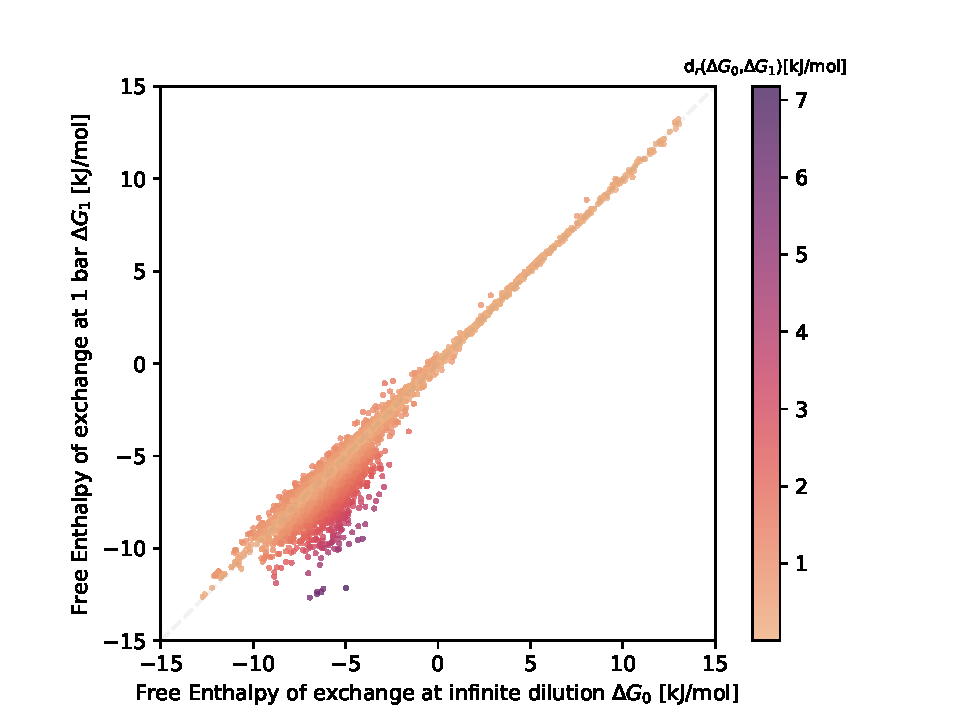
\includegraphics[width=0.5\linewidth]{figures/4-ml/main/Scatterplot_G1_G0.pdf}
  \caption{Comparison between the Gibbs free energy of exchange at low pressure $\Delta G\e{0}$ and ambient pressure $\Delta G\e{1}$ labeled by the relative distance between them. This plot is equivalent to a logarithmic plot of the selectivity at these two pressure conditions.}
  \label{fgr:problem}
\end{figure}

%% Pore size distribution & statistical descriptors
To incorporate information on the pore size diversity of the materials, we carried out statistical measurements on the PSD. By analyzing them, we detected explanatory factors at the origin of the observed selectivity drop. A high degree of multi-modality in the distribution would mean a diverse set of pores, which can lead to a selectivity drop if the pores are significantly different one from another. The more distant is the average pore size from the largest cavity diameter the higher the chance of observing a selectivity drop, because a big difference between the pore sizes bring about a lower selectivity. All these statistics are designed to give as much knowledge as possible on a hypothetical selectivity drop and on the quantitative estimation of its magnitude.

\todo{refer to previous chapter}
%% Energy descriptors statistics
To better quantify the change of selectivity, it could be interesting to give statistics on the distribution of interaction energies for xenon and krypton calculated by our grid algorithm. These statistics include moments of different orders (up to 4) of the energy distribution, which informs on the adsorbate--adsorbent interaction energies in the nanopores at higher loading. The shape of the energy distribution can help assess quantitatively the change in selectivity. We can consider this as a way of compressing the whole energy distribution into a few statistical values, which is a standard method used in the field of data science to tackle distribution data. The same approach has also been applied to the Boltzmann weighted distributions to generate temperature specific descriptors for the energy distributions.

\todo{refer to previous chapter, change text cuz copy paste}
%% 900K gaps
By using different temperatures, we noted that the infinite dilution adsorption enthalpies at higher temperatures can be better correlated to the adsorption enthalpy at ambient pressure. The minimum error was found for the adsorption enthalpy at \SI{900}{\kelvin}, which gives an RMSE of \SI{1.76}{\kilo\joule\per\mole} instead of \SI{2.87}{\kilo\joule\per\mole} for the \SI{298}{\kelvin} case. This new type of descriptor is very interesting since it better performs around the high selectivity region, where the standard Boltzmann average at \SI{298}{\kelvin} loses its accuracy (see Figure~S1). As we can see in the Figure~S7, the exchange free energy at \SI{900}{\kelvin} and the excess of free energy compared to the \SI{298}{\kelvin} case are the second and third most influential descriptors of our ML model. They are complementary to the exchange free energy at \SI{298}{\kelvin} to predict selectivities at higher pressures.

%% conclusion
By combining the above-mentioned features with more standard geometrical descriptors, we trained an ML model for the ambient pressure selectivity that identifies the origins of the selectivity drop and gives promising prediction results.

\subsection{ML model performance}

%% introduction
In this section, we present the performance of the ML model that learned the joint effects of all the newly introduced descriptors to detect and evaluate the observed drop between the easily accessible low-pressure selectivity and the more computationally demanding ambient-pressure selectivity.
A GCMC simulation of a 20-80 xenon/krypton gas mixture takes in average \SI{2,400}{\second} per structure on the CoRE MOF 2019 database, while our grid-based adsorption calculation only takes about \SI{5}{\second} per structure (on a single Intel Xeon Platinum 8168 core at \SI{2.7}{\giga\hertz}). To compute all features needed for our prediction, we would need less than a minute per structure, which is way faster than the 40 minutes required for a GCMC calculation. The ML-based approach has a very clear speed advantage over standard molecular simulations. But to be a good substitute, it needs to keep a good level of accuracy on an unseen set of structures.

\begin{figure}[ht]
\centering
  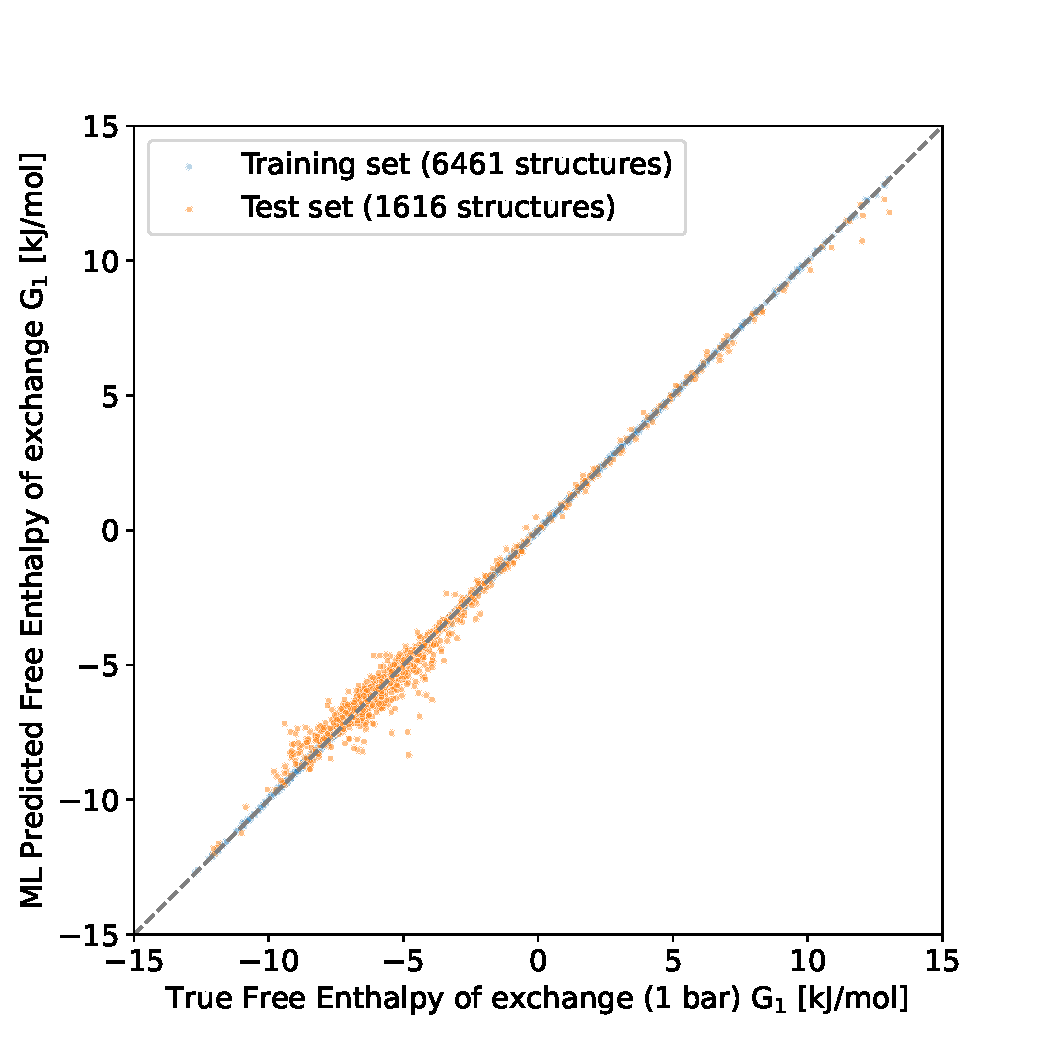
\includegraphics[width=0.5\linewidth]{figures/4-ml/main/Scatterplot_G1_prediction.pdf}
  \caption{Scatter plot of the exchange free energy predicted by the model. There is a good agreement between the predicted and true values. On the test set, there is an RMSE of \SI{0.37}{\kilo\joule\per\mole} and an MAE of \SI{0.21}{\kilo\joule\per\mole}. This plot is equivalent to the scatter plot between the logarithm of the ambient-pressure selectivities (see Figure~S5 of the SI). The corresponding errors for the ambient-pressure selectivity are 2.5 and 1.1 for respectively the RMSE and MAE of the selectivity, and 0.065 and 0.038 for the RMSE and MAE of its base-10 logarithm. }
  \label{fgr:G1_prediction}
\end{figure}

We defined a set of {80\%} randomly chosen structures out of the final dataset to train and fine-tune the parameters of our model. A randomized search over a range of maximum depths, learning rates, sizes of feature samples used by tree and by level, sizes of data sample and alpha regularization parameters has been performed and a set of hyperparameters have been chosen to minimize the average RMSE computed using a 5-fold cross-validation. The ranges used in the randomized search as well as the final hyperparameters set are given in SI. By using this parameterization, our XGBoost model has an RMSE of \SI{0.37}{\kilo\joule\per\mole} and an MAE of \SI{0.21}{\kilo\joule\per\mole} on the exchange Gibbs free energies of the test set of 1,616 structures. If we convert back these results to the selectivity values, the RMSE on the selectivity values would be 2.5 and 0.07 on the logarithm base 10 of the selectivity, which means that the order of magnitude of the selectivity is known with a very good accuracy. To prove that this good performance is not fortuitous, we used a 5-fold cross-validation procedure on the whole dataset and found an average RMSE of \SI{0.36}{\kilo\joule\per\mole} with a standard deviation of \SI{0.01}{\kilo\joule\per\mole}, which is consistent with the performance given by a standard train/test split.

This method can later be used in a screening procedure that relies on cheap descriptors to skim off obviously undesirable structures to only keep the promising structures for the final ML model evaluation. For this is the reason, as previously explained in the methods, only the 3D MOF structures with an LCD above \SI{4}{\angstrom} are kept because they have a positive xenon affinity, which is a necessary condition for a good Xe/Kr selectivity. Our model being very good at predicting the ambient pressure selectivity of structures with good xenon affinity, the proposed screening procedure, illustrated Figure~\ref{fgr:pipeline}, would include (i) a check of the nature of the structure to ensure it is a 3D MOF structure, (ii) then a filter on the LCD value (above \SI{4}{\angstrom}), (iii) a pre-evaluation of the Xe/Kr selectivity at infinite dilution using the grid-based method, and (iv) finally the ML evaluation to keep only structures above a certain threshold of ambient-pressure selectivity (\emph{e.g.} 30). We could eventually evaluate more thoroughly the top structures using GCMC simulations, \emph{ab initio} calculations or adsorption experiments.

\begin{figure}[ht]
\centering
  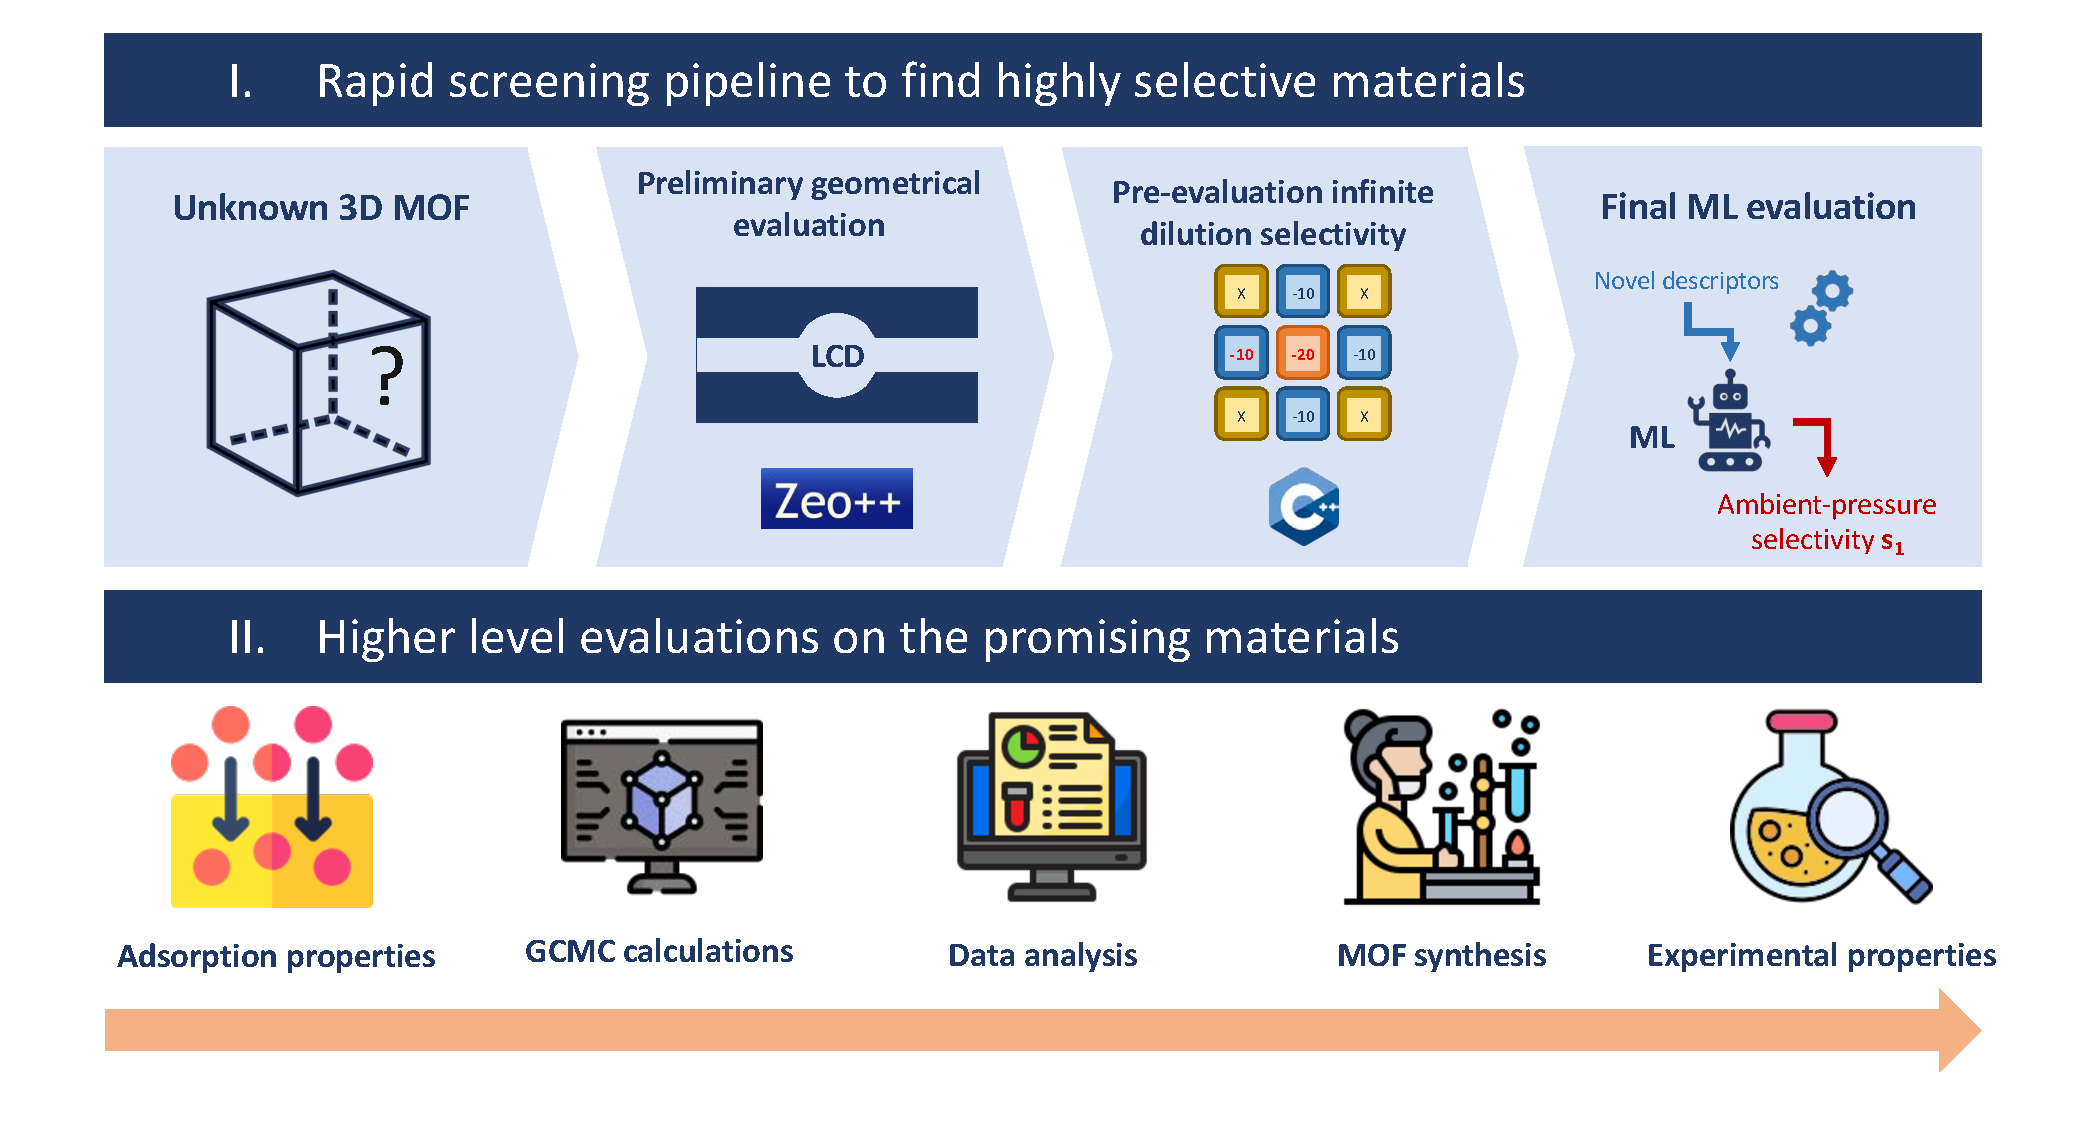
\includegraphics[width=0.99\linewidth]{figures/4-ml/main/pipeline.pdf}
  \caption{An illustration of the screening procedure that could be used to find highly selective materials.}
  \label{fgr:pipeline}
\end{figure}

\section{Opening the Black Box}

%% SHAP intro
To better understand the intuition behind this selectivity drop, we used the SHAP\autocite{SHAP,molnar2020interpretable} library of interpretation models to draw relationships between the descriptors and the predicted ambient-pressure selectivity. This code library is based on the calculation of Shapley values\autocite{shapley1953value} that measure the contribution of each descriptor to the prediction to locally interpret our ML model. This interpretation model untangles the interdependence between the descriptors to extract an individual contribution. To go beyond the local interpretation, we can rapidly compute the Shapley values for the whole dataset using faster algorithms;\autocite{SHAP} scatter plots of the contribution as a function of the descriptor values called SHAP dependence plots can then be drawn to make a more global interpretation of our ML model. Knowing a descriptor value, we could then infer, with a certain level of uncertainty, how it changes the final predicted value, which highlights unknown structure--property relationships. Finally, we can use the mean absolute Shapley values of each feature on the training set to measure the feature importance (see Figure~S7 and S8).

\subsubsection{Explainable AI}

\todo{Present the explainable AI}
The final model is trained on the predefined training set using XGBoost with the fine-tuned hyperparameters. By testing it on the test set, we measure the accuracy of our approach, however, it is interesting to extract chemical insight into the hidden relationship between the predicted value and the descriptors, to better understand the thermodynamic origins of the performance. In this work, we used the Shapley values,\autocite{shapley1953value} a game theory concept developed by Shapley in 1953, to measure the contribution of each descriptor in the predicted value. This tool is used locally to understand for a given structure how their characteristics had contributed to the prediction. To draw structure-property relationships, we would need to use a global interpretation methods such as the SHapley Additive exPlanations (SHAP) method thoroughly detailed in the online book \emph{Interpretable Machine Learning} of Christoph Molnar.\autocite{molnar2020interpretable} The SHAP tool developed by Lundberg and Lee~\autocite{SHAP} is based on a faster algorithm adapted to tree-based ML models like gradient boosting, TreeSHAP, and integrates useful global interpretation modules like SHAP feature importance and dependence plot.

\subsection{Global interpretability}

To rank the descriptors according to their average impact on the magnitude of the model output, we can use the mean absolute Shapley values of each descriptor. The importance plot associated with these values are presented in Figure~S8. Even if the low-selectivity exchange Gibbs free energy has a SHAP importance value way above the others, it only serves as a baseline where a correlation close to the one presented on Figure~\ref{fgr:problem} can be reached; the other descriptors play a major role in moving the outliers of the figure closer to the diagonal line. Energy descriptors play a major role in the model's prediction, and the geometry-based new descriptors, while playing a more secondary role, are key in evaluating the gaps between the low-pressure case with the ambient-pressure one that we are interested in. To dig deeper into the mechanisms that allow the model to predict the selectivity with a very good accuracy --- the RMSE and MAE on the test set's selectivity being respectively $2.5$ and $1.1$ --- we are now going to look into the SHAP dependence plots of each interesting descriptor that plots the contribution to the predicted value as a function of the actual descriptor value.

%% Global Interpretability dependence plot
To make a global interpretation, we applied the partial dependence module provided by the SHAP library on our model. Although other methods to compute dependence plots exist (\emph{e.g.} partial dependence plots),\autocite{molnar2020interpretable} we can keep a good level of consistency between our global and local interpretations by using the same underlying theory. The SHAP dependence plots of all the descriptors of the Figures~S9 and S10, these plots have a rather distinct form, directions and shape, which is encouraging for the interpretability of our model. By looking at the profile of the dependence plots, we can extract valuable information on how the ML model predicts the ambient-pressure selectivity.

%% strong relations
The most important descriptor is obviously the exchange free energy "G\_0" associated to the low-pressure selectivity, its contribution has a very strong positive linear correlation (see Figure~\ref{fgr:pdp_selection}), which gives a base value on top of which the other contributions will either reduce the free energy (more selective) or increase it (less selective). The model can be interpreted as the combination of a baseline combined with smaller tweaks that estimate the magnitude of the deviation from the ideal low dilution case. For instance, the next two descriptors "G\_900K" (\SI{900}{\kelvin} low-pressure exchange free energy) and "G\_Xe\_900K" (\SI{900}{\kelvin} low-pressure xenon adsorption free energy) continue to build up the baseline by providing information on the low-pressure selectivity, but they start giving a glimpse of deviations needed to differentiate between the structures experiencing a drop with the ones that keep their selectivity. As we can see in the SI (Figure~S1 and S2), the thermodynamic quantities at high pressure is closer to the \SI{900}{\kelvin} case than to the ambient temperature one, these two descriptors inform naturally on the selectivity at higher pressure. For "G\_900K" (see Figure~\ref{fgr:pdp_selection}), blue points (corresponding to a "G\_0" of around \SI{-8}{\kilo\joule\per\mole}) can have either negative or negligible contributions depending on the value; values below \SI{-4}{\kilo\joule\per\mole} give a negative contribution with a linear relation, whereas values between $-4$ and \SI{5}{\kilo\joule\per\mole} give constantly almost zero contributions. This type of domain differentiation illustrates how the model can identify structures with a selectivity drop based on the values of a descriptor. We will see more telling examples of how the contribution to the selectivity values are determined using the values of the remaining descriptors.

%% optimal values
The U-shape of some SHAP dependence plots can highlight optimal values for the associated descriptors. For instance, the optimal value of "D\_i\_vdw\_uff298" is around $5.1$ (see Figure~\ref{fgr:pdp_selection}) and the optimal average of pore sizes is around $5.6$. These optimal values match with the physical need of having pores of the size of a xenon to be more attractive to it, which was identified in several papers in the literature. We can note that these values are a bit higher than the ones mentioned in the literature due to the different definition of the atom radii.\autocite{Hung_2021} Moreover, values of "delta\_G0\_298\_900" between $4$ and \SI{6}{\kilo\joule\per\mole} (see Figure~\ref{fgr:pdp_selection}) have a higher chance of giving a negative contribution, which means a lower ambient-pressure selectivity. These sweet spots constitute valuable hints to tell the truly selective materials from the others. Some SHAP dependence plots have a rather linear domain for the most selective structures (in blue) --- the difference of pore volumes between Xe and Kr sized probes "delta\_VF\_18\_20" have a good linear contribution (see Figure~\ref{fgr:pdp_selection}), which means that the lower the more selective the structure will be. The same can be said for the standard deviations of the PSD "pore\_dist\_std" and of the Boltzmann weighted krypton interaction energies distribution "enthalpy\_std\_krypton". The optimal values for these descriptors are zero, the closest to zero it is the more negative the contribution will be and the more selective the structure at ambient pressure.

%% optimal domains (weak relations)
Sometimes the optimal values are not around well-identified values but are contained within larger domains with threshold values separating them. For instance, the difference between the LCD and the average pore size "delta\_pore" has a threshold value around \SI{0.3}{\angstrom} below which the contribution for the most selective structures (blue) is negative (see Figure~\ref{fgr:pdp_selection}); even though no clear correlations can be found, we can at least find a threshold value (about $0.23$) below which there is higher probability of having a high ambient-pressure selectivity. The same type of domain splits can be found for the average of krypton interaction energies distribution "mean\_grid\_krypton" (at around $15$), the Boltzmann weighted xenon interaction energies distribution "enthalpy\_std\_xenon" (at around $2.5$), the difference of exchange entropic term between the ambient temperature "delta\_TS0\_298\_900" (at around $3$) and high temperature and the effective number associated to the PSD "pore\_dist\_neff" (at around $2.3$). These domains separate structures that are selective at low pressure, which is key to telling apart the structures with a selectivity drop at ambient pressure from the ones without.

\begin{figure}[ht]
\centering
  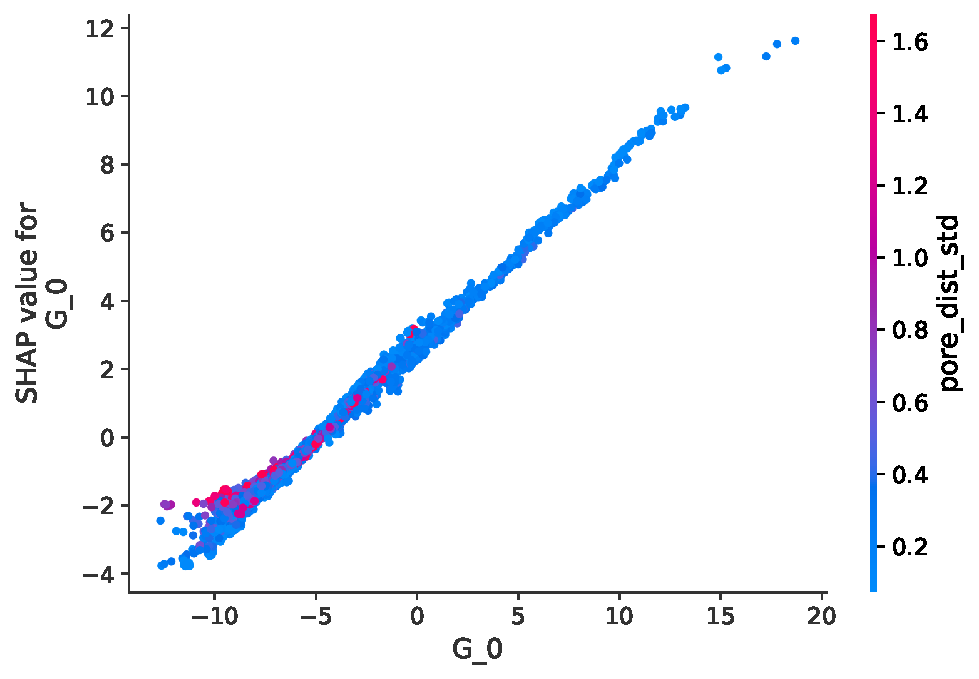
\includegraphics[width=0.32\linewidth]{figures/4-ml/SDP/G_0.pdf}
  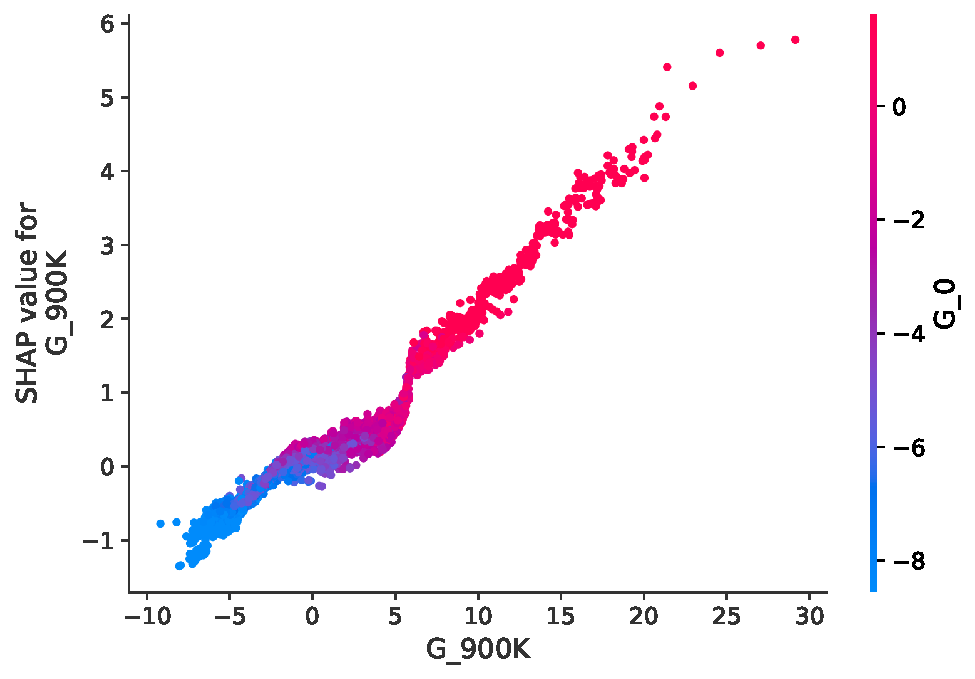
\includegraphics[width=0.32\linewidth]{figures/4-ml/SDP/G_900K.pdf}
  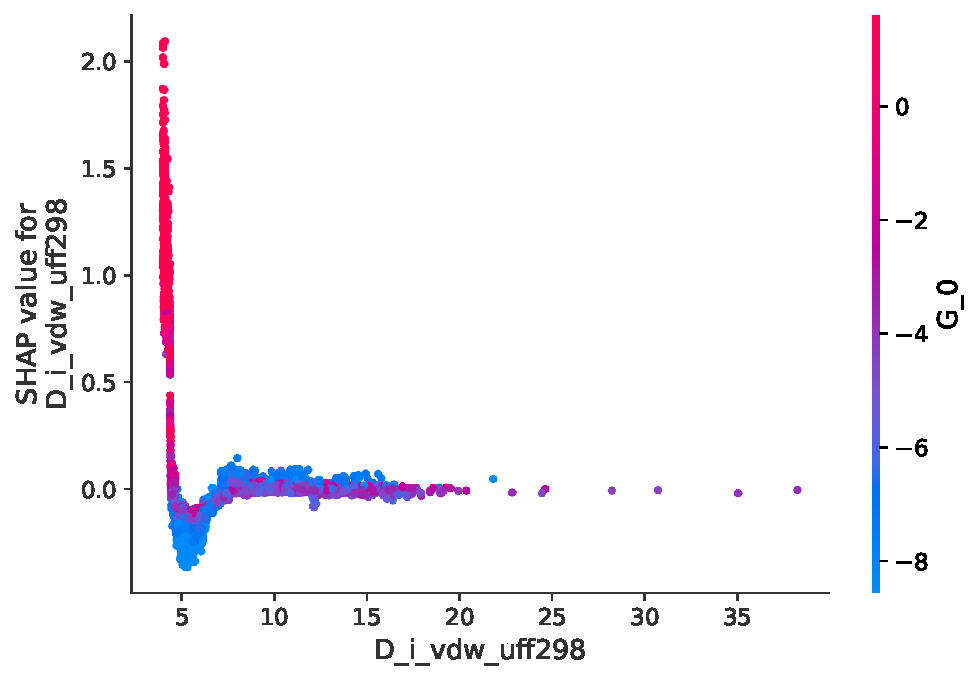
\includegraphics[width=0.32\linewidth]{figures/4-ml/SDP/D_i_vdw_uff298.pdf}
  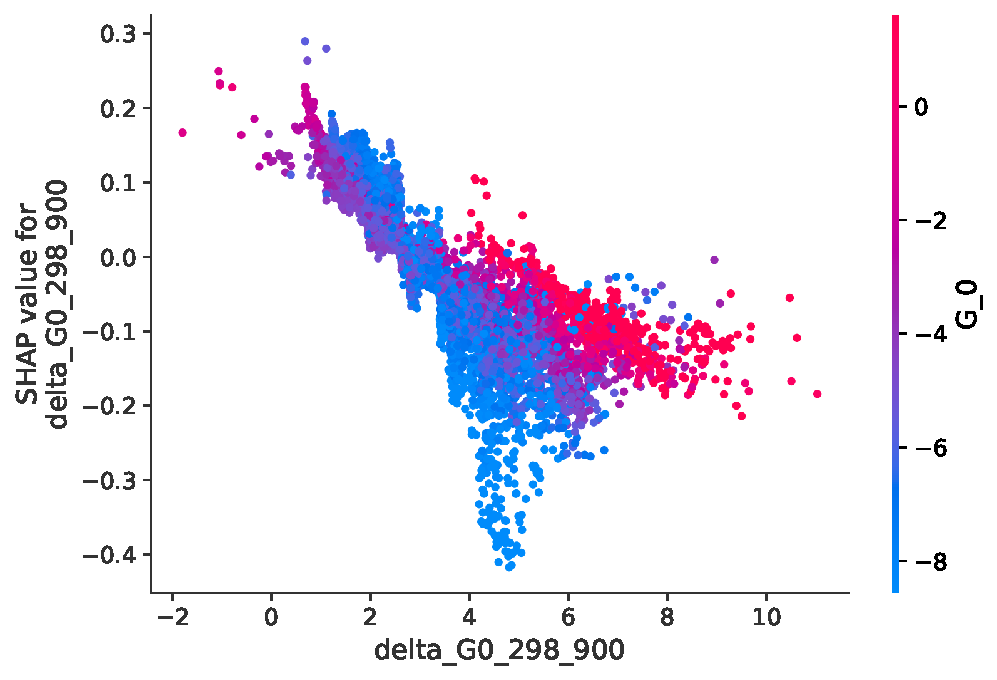
\includegraphics[width=0.32\linewidth]{figures/4-ml/SDP/delta_G0_298_900.pdf}
  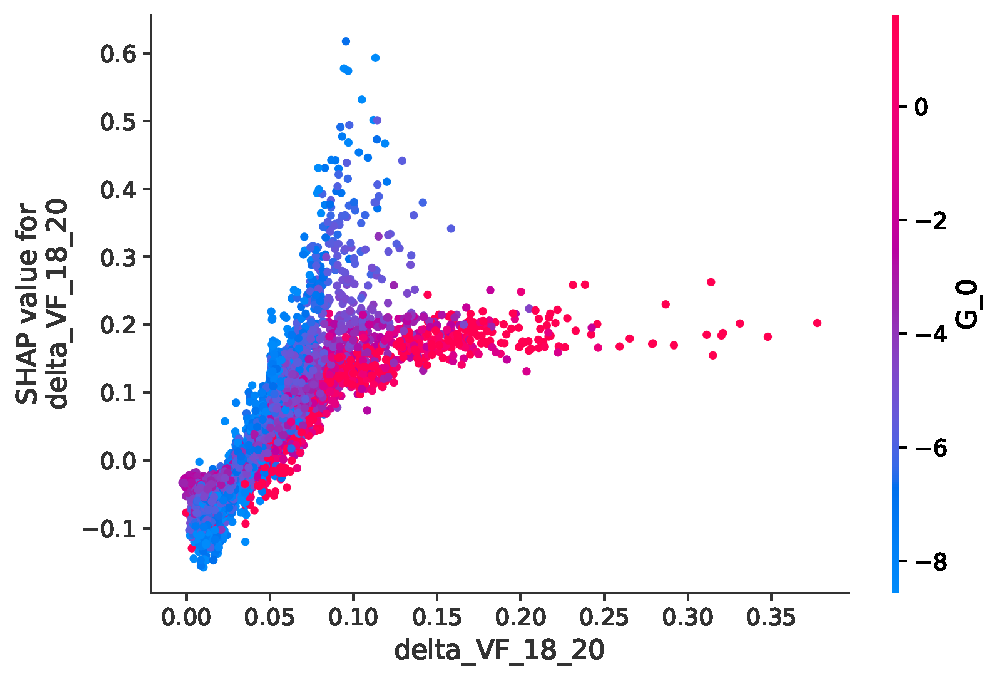
\includegraphics[width=0.32\linewidth]{figures/4-ml/SDP/delta_VF_18_20.pdf}
  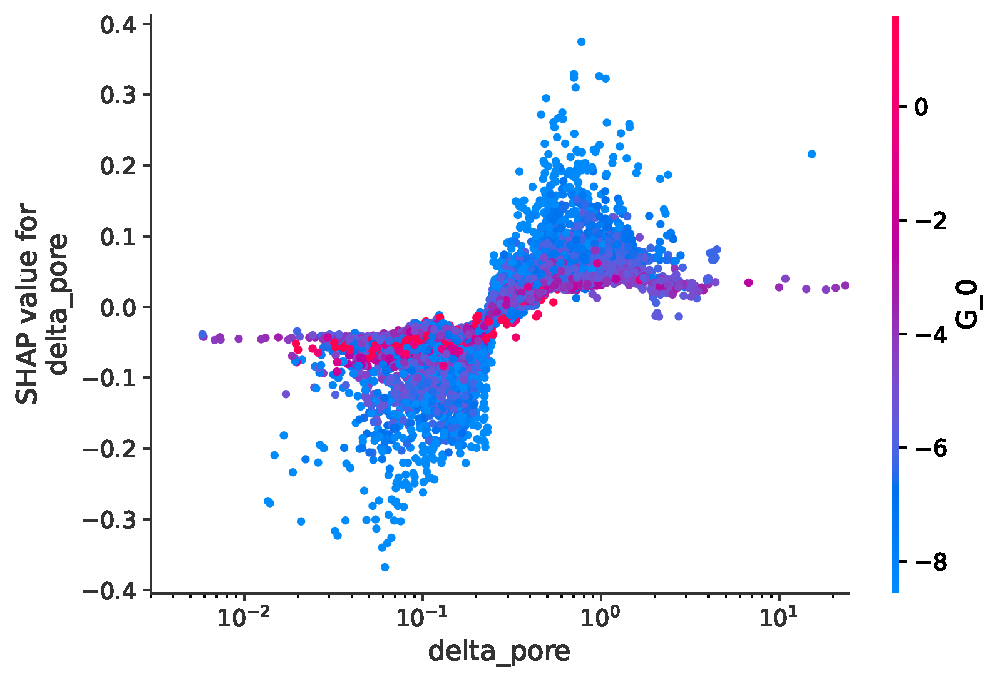
\includegraphics[width=0.32\linewidth]{figures/4-ml/SDP/delta_pore.pdf}
\caption{Some SHAP dependence plots that are analyzed in the main article. The 18 top descriptors' SDPs can be found in the SI. }
  \label{fgr:pdp_selection}
\end{figure}

\subsection{Local interpretability}

%% local interpretation
To put into practice our previous analysis, let's look at some archetypal structures and how the model predicted the selectivity based on the descriptor values. We chose two MOF structures from the test set, their CSD code being respectively VIWMIZ and BIMDIL. Both structures are selective at low pressure but the first one decreases in selectivity while the other maintains it at ambient pressure. It will be interesting to see what the model does to tell apart these two completely different behaviors.

VIWMIZ is part of the highly selective structures that experience a selectivity drop at ambient pressure. If we convert back the free energy values to selectivity values, its selectivity is $62.8$ at infinite dilution and $14.5$ at ambient pressure. The ML model manages to give a close prediction of $12.0$ for the ambient-pressure selectivity based on the given values of the descriptors. If we only look at "G\_0", it has one of the most negative values, which explains the rather high negative contribution of $-1.81$. However, the $-0.57$ contribution of "G\_900K" is rather low compared to other materials (see Figure~\ref{fgr:pdp_selection}), since a value of $-4.05$ is not the most negative considering all structures. On the other hand, the remaining descriptors have values in the domain of positive contributions, which lead to the drop of the selectivity. For example, the difference of pore sizes "delta\_pore" has a value of \SI{1.38}{\angstrom} (above the threshold of \SI{0.23}{\angstrom}), which contributes $+0.25$ to the predicted selectivity and is consistent with the value ranges of the associated dependence plot. By reporting the values to the dependence plots, the same analyses can be made on the other positive contributions of the Figure~\ref{fgr:contribution}: "pore\_dist\_std" is above the threshold of $0.4$, "enthalpy\_std\_krypton" is above \SI{2.5}{\kilo\joule\per\mole}, "pore\_dist\_neff" is above $2.3$, "delta\_TS0\_298\_900" is below \SI{3}{\kilo\joule\per\mole} and "enthalpy\_modality" is around $0.75$ where positive contributions are more commonly observed. However, the "delta\_G0\_298\_900" value is a bit too close to its optimal value, which explains its negative contribution in this particular prediction. The rest of the features have almost negligible contributions and are detailed in the Figure~S11. By analyzing the contributions of each descriptor to the prediction given by our model, we can understand the underlying features of the VIWMIZ structure that explains the selectivity drop at higher pressure. The shape of the xenon and krypton energy distributions ("enthalpy\_std\_krypton" and "enthalpy\_modality") and of the PSD ("pore\_dist\_std" and "pore\_dist\_neff" ) as well as the void fraction difference "delta\_pore" are key descriptors at the origin of the lower selectivity at ambient pressure compared to the ideal infinite dilution case. Intuitively, one can easily understand that effective number of pores exceeding 2 can mean the presence of different pore sizes, which is consistent with the presence of pores that are less attractive to the xenon and leads necessarily to less selectivity. The previous statement is also very much consistent with a high standard deviation of the PSD or the Boltzmann weighted krypton interaction energy distribution. One can also conceive that a much larger difference between the average pore size and the LCD could mean a high disparity in pore sizes that leads to the presence of larger pores more and more loaded as the pressure rises.
The entropic term is however way more complex to interpret and opens unexplored ways of tackling the problem of selectivity drop at higher pressure unraveled by our previous study\autocite{Ren_2021}.

\begin{figure}[ht]
    \centering
    \begin{subfigure}[b]{0.47\textwidth}
      \centering
      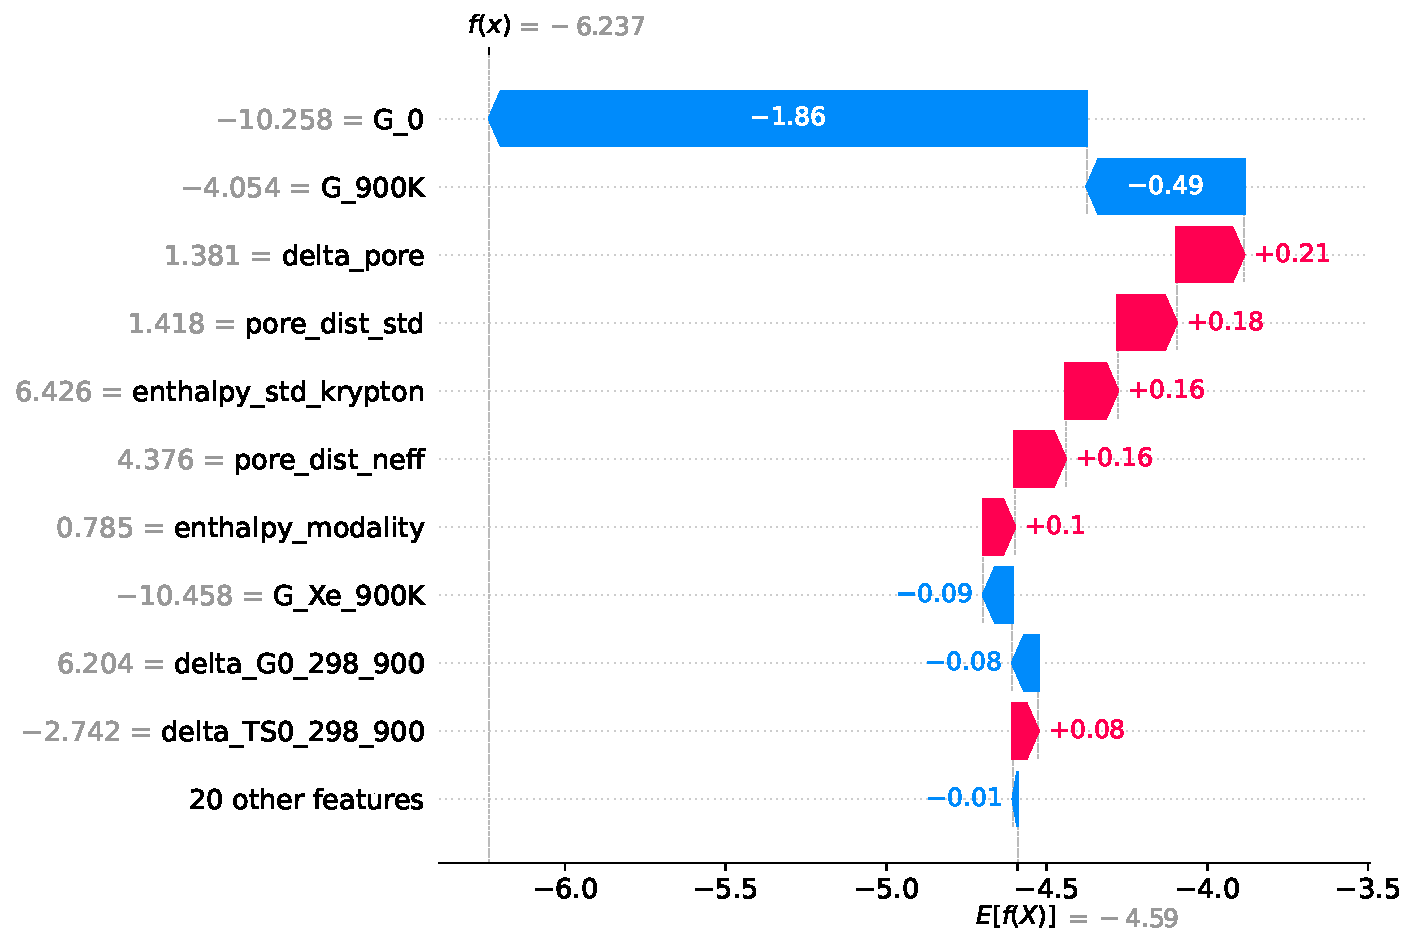
\includegraphics[width=\textwidth]{figures/4-ml/main/VIWMIZ_clean.pdf}
      \caption{VIWMIZ: true $\Delta\e{exc} G_1=-6.63$}
    \end{subfigure}
         \hfill
    \begin{subfigure}[b]{0.47\textwidth}
      \centering
      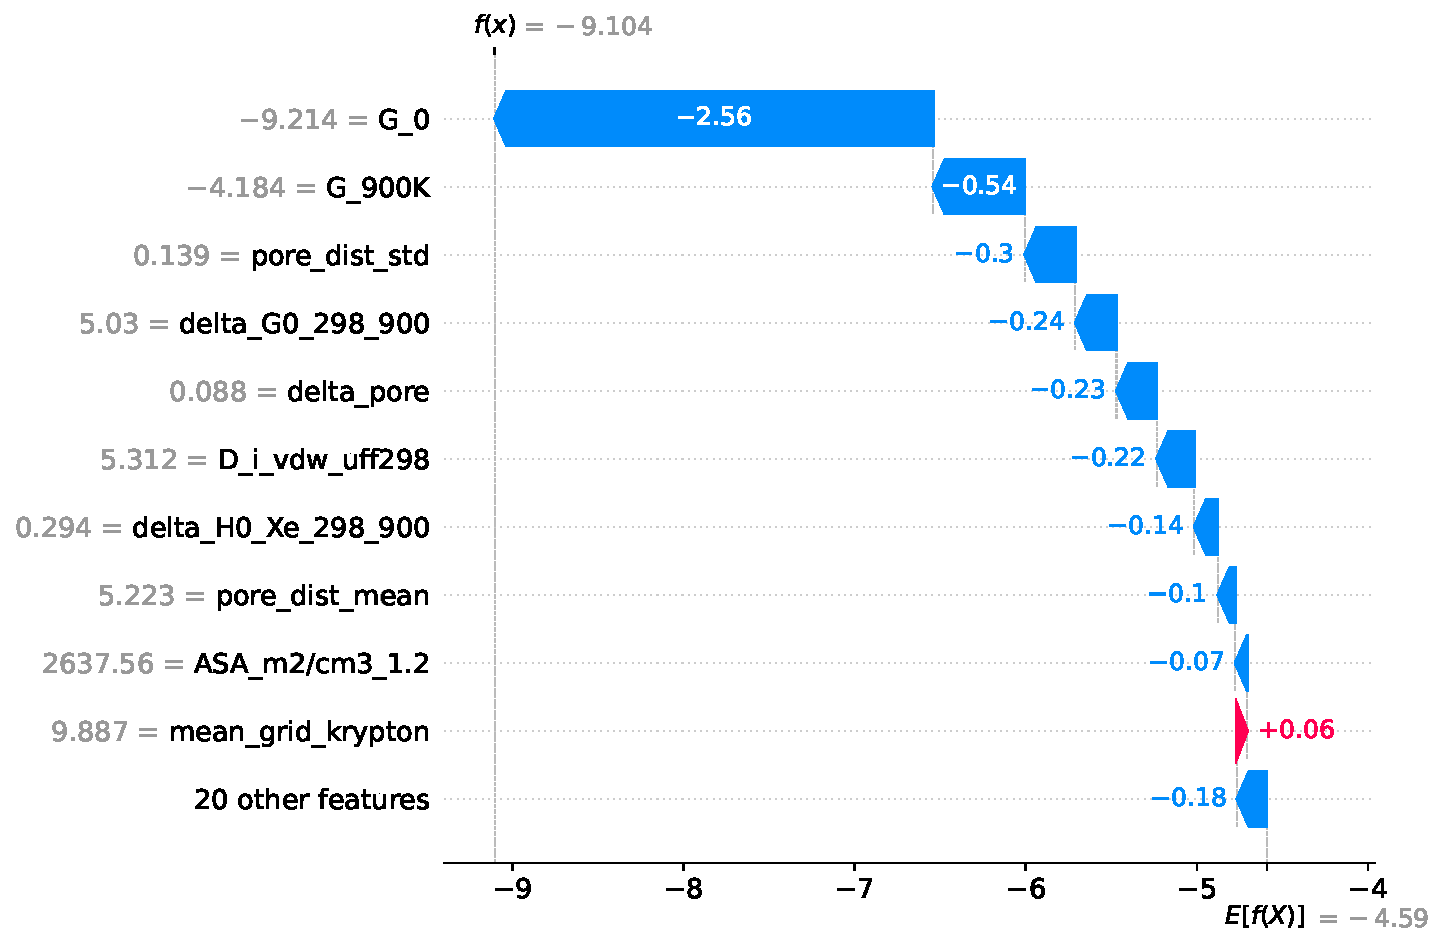
\includegraphics[width=\textwidth]{figures/4-ml/main/BIMDIL_clean.pdf}
      \caption{BIMDIL: true $\Delta\e{exc} G_1=-9.20$}
    \end{subfigure}
  \caption{Main contributions of the descriptors on the selectivity prediction of two archetypal examples. The descriptor labels used are detailed in the Table~S1 and S2 of the SI.}
  \label{fgr:contribution}
\end{figure}

The second structure BIMDIL is also among the most selective with a selectivity at low pressure of $41.0$, while maintaining it to $41.2$ at ambient pressure. The model manages to predict this stability of the selectivity by giving a value of $40.0$. Consequently, the first contribution of "G\_0" is among the most negative ones and set a baseline of $-2.4$ for the upcoming contributions. The contributions of "G\_900K" and "G\_900K" are not the highest possible but they continue to lower down the value of the predicted selectivity. It is the joint contributions of the other descriptors that will really discriminate between the two structures and decide why this one will keep its selectivity. Unlike the previously analyzed structure, this one has a "delta\_pore" value below \SI{0.3}{\angstrom}, which explains the negative Shapley value it has for our prediction. The contribution of "delta\_G0\_298\_900" that was only a little negative for the other one, is now playing a major role since it is right within the range of between $4$ and \SI{6}{\kilo\joule\per\mole} (see Figure~\ref{fgr:contribution}). We can also verify that "pore\_dist\_std" is now below the threshold instead of being above for the other structure. We can confirm that the other contributions are also following the rules implied by the SHAP dependence plots, no apparent anomalies are detected, and the joint efforts of all the descriptors tend to give a lower free energy value, which leads to the conservation of the selectivity value at higher pressure. The set of descriptor values is clearly very different from the previous structure, many values are in opposite contribution domains, which explains how the model manages to disentangle the highly selective structures to find out the ones that would keep their selectivity at higher pressure.

%% conclusions + sum-up of some qualitative rules
These two examples allow us to understand a bit more how the model tells apart the structures that will lose selectivity at higher pressure from the ones that will not. Most of the dependence plots can give very strong association between the descriptors and their effects; the outliers are rare enough that the inner logic of our model can be understood. As developed previously, the first three descriptors set a baseline on few information on the eventual drop of selectivity; then the other descriptors contribution is either positive, negligible or negative depending on the domain of values the descriptor is in. For instance, the average pore size and the largest cavity diameter need to be around very specific values to maximize the chance of keeping the selectivity at higher pressure, which was highlighted by previous works that emphasize on the importance of pore sizes close to the size of xenon for Xe/Kr separation.\autocite{Simon_2015, Ren_2021} The difference of entropy between the ambient temperature and \SI{900}{\kelvin} is surprising descriptor that separates selective structures depending on whether its value is within a given range. The difference of void fraction occupied by xenon and krypton is also very interesting since it affects the selectivity differently depending on whether it is highly selective or not, and the contribution is more or less proportional to its value. Different ways of measuring the disparity of the PSD and interaction energy distribution are key in sorting highly selective structures (in blue on the dependence plot Figure~\ref{fgr:pdp_selection}) between the ones maintaining their performance and the ones decreasing in selectivity. Among others, we can find the difference between the average pore size and the LCD, as well as the standard deviation of the PSD or of the Boltzmann weighted energy distribution that would behave very differently according to the domain in which the value lies. The SHAP dependence plots, partially plotted in the main text and entirely available in the SI, are very valuable reading grid to understand the mechanisms behind our ML model and more broadly to what it understood from the origins of Xe/Kr separation.

\subsection{Conclusions and perspectives}

In order to better understand separation processes inside nanoporous materials, we performed a machine learning prediction of Xe/Kr ambient-pressure selectivity that is faster than standard GCMC calculations. For MOF structures of the CoRE MOF 2019 database, a xenon/krypton selectivity evaluation would take less than a minute, while an equivalent GCMC calculation takes around \SI{40}{\minute}. Unlike most of the selectivity predictions of the literature, we chose to predict a selectivity in the logarithmic scale, because it focuses more on the order magnitude than the exact value of the selectivity of highly selective materials. Moreover, the conversion to an exchange Gibbs free energy allows a more thermodynamic approach based on enthalpy, entropy and free energy values. The challenge was then to predict a free energy equivalent of the ambient-pressure selectivity by using the low-pressure selectivity along with key energy, geometrical and chemical descriptors. The final, fully optimized ML model performs very well with an RMSE of \SI{0.36}{\kilo\joule\per\mole}, which corresponds to a $0.06$ RMSE on the base-10 log of the selectivity.

One of our more specific goals was to uncover underlying reasons of a selectivity drop at high pressure observed on some highly selective materials at low pressure. Previous studies found that a high diversity of pore sizes and channel sizes that favor adsorbate reorganizations could be at the origin of this phenomenon.\autocite{Ren_2021} By applying interpretability tools, we found quantitative factors that explain the conservation or the drop of the selectivity for highly selective materials. Depending on energy averaging at \SI{900}{\kelvin}, on statistical characterizations of the energy or pore size distributions, and on the difference of volumes occupiable we have a structure either with a selectivity similar to the low-pressure case or that is less selective at higher pressure. All the quantitative rules are contained in a complex ensemble of decision trees constructed by our XGBoost model, and they can be extracted to build rule of thumbs in order to back our intuition on the Xe/Kr selectivity in MOF structures.

%% Framework could be reproduced for other type of applications
The final ML model can be used in a well-designed workflow to find the best performing materials. For instance, we could filter out the structures with pores that cannot fit a xenon in, then we could use a first calculation of the low-pressure selectivity to filter out the selectivity below a given threshold. Finally, we can use the model to remove the structures that would experience a selectivity drop. We tested our methodology on the Xe/Kr separation as proof of concept since it is one of the simplest adsorption systems (monoatomic species with no electrostatic interactions). A similar approach can be generalized to other separation applications by calculating the infinite dilution energies with a more standard method (\emph{e.g.} Widom's insertion) and by adjusting the descriptor definitions to fit the adsorbates of interest.

%% Drawbacks + perspectives
This study ambitions to add new descriptor ideas to help the development of ever more efficient screening methodologies to find the best materials for target applications. However, like many other studies on the topic, this one also relies on a few strong assumptions --- the simulations are performed in rigid frameworks with non-polarized classical force fields. As suggested in the literature, the most selective materials ever synthesized for Xe/Kr separation are all based on the effect of open-metal sites that uses the difference of polarizability between the two molecules to efficiently separate them.\autocite{Li_2019, Pei_2022} Moreover, the structures can be made flexible using flexible force fields with adapted simulation methodologies\autocite{Bousquet2012} or by using multiple rigid simulations of snapshots from NPT simulations\autocite{Witman_2017}.
It would be possible to improve the simulations at the cost of CPU times, if we coupled it with a reduction of simulation time like the one presented in this article. The quest of ever-faster evaluation tools will allow us to investigate more complex properties and uncover structures with ever more interesting characteristics.

\textbf{Data Availability:} \url{}

\OnlyInSubfile{\printglobalbibliography}

\end{document}
